\chapter{Kravspecifikation}

\begin{longtabu} to \linewidth{@{}l l l X[j]@{}}
    Version &    Dato &    Ansvarlig &    Beskrivelse\\[-1ex]
    \midrule
\label{version_Systemark}
\end{longtabu}


\section{Indledning}
 Et blodtryksmålingssytem er blevet udarbejdet, der helt generelt er opbygget af en hardware del og en software del. Hardware delen er opbygget af en forstærker, transducer og analogt filter hvis formål er at kunne forstærke og filtrerer blodtrykssignalet og software delen kalibrerer, nulpunktsjusterer og analysere signalet samt viser signalet grafisk på en brugergrænsefalde. \\
 Kravspecifikationen vil beskrive, produktets kunnen ud fra nogle opstillede funktionelle og ikke funktionelle krav til systemet. De ikke funktionelle krav er krav, der er opstillet til selve systemet og de funktionelle krav er beskrevet i use cases, som omhandler systemts aktiviteter i forhold til aktører og mål. 


\section{Funktionelle krav}
\subsection{Aktør-kontekst diagram}

\begin{figure}[H]
	\centering
	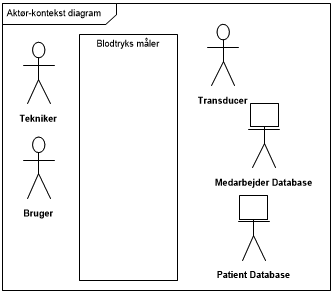
\includegraphics[width=0.5\textwidth]{Figurer/ISE/aktdiagram2}
	\caption{Aktør-kontekst diagram}
	\label{Aktdiagram}
\end{figure}


\subsection{Aktørbeskrivelse}

\begin{longtabu}to \linewidth{@{}l l X[j]@{}}
	{\large \textbf{Aktørnavn}} & {\large \textbf{Type}} & {\large \textbf{Beskrivelse}}\\ \toprule
	Bruger & Primær & Brugeren er den aktør der foretager blodtryksmålingerne. Brugeren er en person der har kendskab til systemet, samt tilladelse til at benytte systemet. Fx en læge, anestesi sygeplejerske \\
	Tekniker & Primær & Tekniker er den aktør der foretager den årlige kalibrering af systemet. Teknikeren er en person der har kendskab til den tekniske del af systemet. Fx. medicotekniker på et sygehus\\
	Transducer & Sekundær & Det er tranduceren, der leverer blodtryksmålingen til systemet\\
	Medarbejder database & Sekundær & Medarbejder databasen er det sted, hvor medarbejderens log ind valideres \\
	Pateint database & Sekundær & Patient databasen er det sted, hvor blodtryksmålingens data gemmes og patientens CPR nummer valideres \\ \bottomrule
\caption{Aktørbeskrivelse}
\label{Aktoerbeskrivelse}
\end{longtabu}

\section{Use cases}
\subsection{Use case diagram}
\begin{figure}[H]
	\centering
	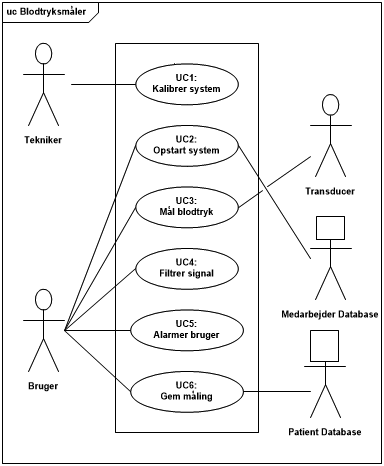
\includegraphics[width=0.7\textwidth]{Figurer/ISE/UcDiagram2}
	\caption{Use case diagram}
	\label{UC diagram}
\end{figure}

\begin{longtabu} to \linewidth{@{}l r X[j]@{}} %UC1%
    {\large \textbf{Use Case 1}} && \\
    \toprule
    Navn &&    Kalibrer system\\
    Use case ID &&    1\\
    Samtidige forløb &&    1\\
    Primær aktør &&    Tekniker\\
    Initialisere &&    Tekniker\\
    Mål && Tekniker ønsker at foretage kalibrering\\
    Forudsætninger &&  \\
    Resultat &&    Systemet er kalibreret                     \\ \midrule
    Hovedforløb &    1. &    Tekniker påtrykker systemet tre kendte tryk  \\
    			&    2. &    Tekniker aflæser responserne  \\ 
    			&    3. &    Tekniker noterer afvigelser fra de kendte tryk \newline [\textit{3.a Der er ingen afvigelser}]  \\
    			&    4. &    Tekniker kalibrerer afvigelsen  \\ \midrule 		
    Undtagelser &    3.a & Use case afsluttes \\ \bottomrule
\caption{Fully dressed Use Case 1}
\label{UC1}
\end{longtabu}

\begin{longtabu} to \linewidth{@{}l r X[j]@{}} %UC2%
    {\large \textbf{Use Case 2}} && \\
    \toprule
    Navn &&    Opstart system\\
    Use case ID &&    2\\
    Samtidige forløb &&    1\\
    Primær aktør &&    Brugeren\\
    Sekundær aktør && Database\\
    Initialisere &&    Brugeren\\
    Mål && Systemet er opstartet\\
    Forudsætninger &&  Use case 1 er gennemført.\\
    Resultat &&    Systemet er nulpunktsjusteret og brugeren er klar til at blive forbundet til systemet\\
    \midrule
    Hovedforløb &    1. &    Brugeren indtaster login-oplysninger og trykker på "Log ind"\--knappen. Systemet tjekker i databasen om oplysninger er gyldige \newline [1.a \textit{Forkert login}]\\
    	&			2. & Brugeren trykker på "nulstil"\--knappen. Systemet laver nulpunkts justering \newline [\textit{2.a Systemets nulpunktjustering er ikke korrekt}] \\ \midrule
    Undtagelser &    1a. & Besked om forkert login vises. Use Case fortsættes fra punkt 1     \\ 
    	&			2.a & Indikation om at systemet ikke er nulpunktjusteret vises. Use Case fortsættes fra punkt 2 \\ \bottomrule    
\caption{Fully dressed Use Case 2}
\label{UC2}
\end{longtabu}


\begin{longtabu} to \linewidth{@{}l r X[j]@{}} %UC3%
    {\large \textbf{Use Case 3}} && \\
    \toprule
    Navn &&    Mål blodtryk\\
    Use case ID &&    3\\
    Samtidige forløb &&    1\\
    Primær aktør &&    Brugeren\\
    Initialisere &&    Brugeren\\
    Mål && Blodtryksmåling kører\\
    Forudsætninger && UC2 er gennemført\\
    Resultat &&    Blodtrykket vises i kontinuerlig graf, systolisk og diastoliske blodtryk vises grafisk, samt puls vises grafisk                     \\ \midrule
    Hovedforløb &    1. &    Brugeren trykker på "start"\--knappen i blodtryksvindue\\
    			& 	 2. & Transduceren måler blodtryk\\
    			&	 3. & Systemet modtager blodtryksmåling fra transduceren\\
    			& 	 4. & Blodtrykgraf, systolisk, diastolisk og puls vises grafisk i blodtryksvinduet\\ \midrule               
    Undtagelser &     &  \\ \bottomrule
\caption{Fully dressed Use Case 3}
\label{UC3}
\end{longtabu}

\begin{longtabu} to \linewidth{@{}l r X[j]@{}} %UC4%
    {\large \textbf{Use Case 4}} && \\
    \toprule
    Navn &&    Filtrer signal\\
    Use case ID &&    4\\
    Samtidige forløb &&    2\\
    Primær aktør &&    Brugeren\\
    Initialisere &&    Brugeren\\
    Mål && Brugeren ønsker at foretage en digital filtrering\\
    Forudsætninger && UC2 er gennemført\\
    Resultat &&    Det filtrerede signal vises i blodtryksgrafen                    \\ \midrule
    Hovedforløb &    1. &    Brugeren trykker på "Til"\--knappen under filtrer\\
    			&	 2. & 	 Systemet filtrerer signalet\\
    			&	 3. 	&	 Det filtrerede signal vises i blodtryks vindue \\ \midrule               
    Undtagelser &    \\ \bottomrule
\caption{Fully dressed Use Case 4}
\label{UC4}
\end{longtabu}

\begin{longtabu} to \linewidth{@{}l r X[j]@{}} %UC5%
    {\large \textbf{Use Case 5}} && \\
    \toprule
    Navn &&    Alarmer bruger\\
    Use case ID &&    5\\
    Samtidige forløb &&    2\\
    Primær aktør &&    Brugeren\\
    Initialisere &&   Brugeren\\
    Mål && Systemet kan alarmere bruger ved for højt/lavt blodtryk\\
    Forudsætninger && UC2 er gennemført\\
    Resultat &&    Systemet alarmerer bruger                    \\ \midrule
    Hovedforløb &    1. &    Brugeren tilpasser diastoliske og systoliske grænseværdier ud fra patientens blodtryk\\ 
    			& 	 2. & 	Systemet tjekker om grænseværdier er overskredet\\ 
    			&	 3. & 	Målte blodtryk overskrider valgte grænseværdier\newline [\textit{3.a Målte blodtryk overskrider ikke valgte grænseværdier}]\\ 
    			& 	 4. & 	Alarm startes \newline [\textit{4.a Bruger udskyder alarm}]\\ \midrule            
    Undtagelser &    3.a & Use case fortsættes fra punkt 2 \\ 
    			&	 4.a & Alarm udskydes med 3 minutter og use case starter fra punkt 2 igen\\ \bottomrule
\caption{Fully dressed Use Case 5}
\label{UC5}
\end{longtabu}


\begin{longtabu} to \linewidth{@{}l r X[j]@{}} %UC6%
    {\large \textbf{Use Case 6}} && \\
    \toprule
    Navn &&    Gem måling\\
    Use case ID &&    6\\
    Samtidige forløb &&    1\\
    Primær aktør &&    Brugeren\\
    Mål &&    Brugeren ønsker at afslutte systemet og gemme måling\\
    Forudsætninger && UC3 er gennemført\\
    Resultat &&    Blodtryksmålingens data er gemt i database og bruger er logget ud af systemet                    \\ \midrule
    Hovedforløb &    1. &    Brugeren trykker på "Gem og afslut"\--knappen. "Gemme"\--vindue åbnes. \newline [1.a \textit{Bruger ønsker ikke at afslutte}]\\  						 	
                &    2. & Brugeren indtaster CPR-nr og trykker på "\\
                &    3. & Brugeren trykker på "gem og afslut"\--knappen. Systemet logger ud og afsluttes\\
                \newline [3.a \textit{CPR-nr er ikke gyldigt}]	\\ \midrule                
    Undtagelser &    1.a. & Bruger trykker på "Annuller"\--knappen. Use Case 3 \\ 
    			&	3.a. &  Besked om at CPR-nummer ikker gyldigt, vises. Nyt CPR-nummer indtastet. Use Case fortsættes for punkt 2\\ \bottomrule
    		
\caption{Fully dressed Use Case 6}
\label{UC6}
\end{longtabu}

\section{Ikke-funktionelle krav}
\subsection{(F)URPS+}
MoSCow er angivet i parentes ved hhv. M, S, C og/eller W, for Must, Should, Could og Won't\\


\textbf{Functionality}\\
\begin{enumerate}
	\item (M) Brugeren skal kunne starte en ny måling indenfor XX sekunder efter opstart af programmet \\
	\item (M) Systemet skal kunne kalibrere blodtrykssignalet\\
	\item (M) Systemet skal kunne foretage en nulpunktsjustering\\
	\item (M) Systemet skal kunne forstærke signalet fra transduceren (INDSÆT VÆRDI)\\
	\item (M) Systemet skal kunne filtrere signalet med det indbyggede analoge antialiaserings filter med en båndbredde på 50 Hz \\
	\item (M) Programmet skal kunne vise blodtrykket som funktion af tiden\\
	\item (M) Programmet skal kunne vise blodtrykssignalet kontinuert\\
	\item (M) Programmet skal programmeres i C\#\\
	\item (M) Programmet skal kunne lagre de målte data i en database\\
	\item (M) Programmet skal kunne filtrere blodtrykket via et digitalt filter\\
	\item (S) Programmet bør kunne afbildede både systolisk og diastolisk blodtryk med tal\\
	\item (S) Programmet bør kunne måle puls\\
	\item (C) Programmet kan angive pulsslag med bip-lyde med varighed af 100ms og en frekvens på 850 Hz\\
\end{enumerate}

\textbf{Usability}\\
\begin{enumerate}
	\item (M) Blodtrykstallene der udskrives på brugergrænsefladen er røde\\
	\item (S) Pulsmålingen burde kunne udskrives på brugergrænsefladen med grønne tal\\
	\item (M) Brugeren skal kunne starte en måling maksimalt 20 sekunder efter opstart\\
Knapper??\\
Billede af brugergrænsefladen indsættes\\	
\end{enumerate}

\textbf{Reliability}\\
\begin{enumerate}
	\item (M) Systemet skal kunne køre uden fejl i et år\\
	\item (M) Systemet skal have en ”mean time to restore” på højest 24 timer\\
	\item Systemet får herved en tilgænglighed beregnet ved \begin{align}
Availability = \frac{MTBF}{MTBF+MTTR} = \frac{365}{365+1} = 0,997 = 99,7 \%
\end{align}\\
\end{enumerate}

\textbf{Performance}\\
\begin{enumerate}
	\item (S) Systemet bør kunne gemme data på 5 sekunder +/-10\%\\
\end{enumerate}

\textbf{Supportability}\\
\begin{enumerate}
	\item (M) Softwaren er opbygget af trelagsmodellen\\
\end{enumerate}




















